\subsection{Clustering using \acs*{optics}}\label{subsec:impl-optics}

\begin{figure}[!htp] % htp = hier (h), top (t), oder auf einer eigenen Seite (p).
    \centering
    \includesvg[width=1\textwidth]{images/OPTICS/OPTICS_procedure.svg}
    \caption[\acs*{optics} procedure]{The first page of each document is converted to an image.
    The image is preprocessed, i.e.\ conversion to greyscale and resizing.
    }
    \label{fig:OPTICS_procedure}
\end{figure}

Similar to the approach from \citeauthor{OPTICS1999}, \ac{optics} is used to cluster the images of the first page of documents in this work.
The procedure is displayed in \autoref{fig:OPTICS_procedure}.
There are two different preprocessing approaches:
\begin{enumerate}
    \item \label{pt:32}The images are first preprocessed to 32x32 normalized greyscale pixels (cf. \cite{OPTICS1999}) 
    as visualized in \autoref{fig:preprocessed_docs_32x32}
    and afterwards compressed to 13-dimensional vectors using \ac{pca}.
    \item \label{pt:eigendocs}The technique \eigendocs{} from \autoref{subsec:eigenface} 
    is used to compress the images to 13-dimensional normalized greyscale images as displayed in \autoref{fig:preprocessed_docs_eigendocs}.
\end{enumerate}

% reachability plot
\begin{figure}[!htp]%
    \centering
    \subfloat[\centering The reachability plot of the documents preprocessed according to \autoref{pt:32} (cf. \cite{OPTICS1999}).]{{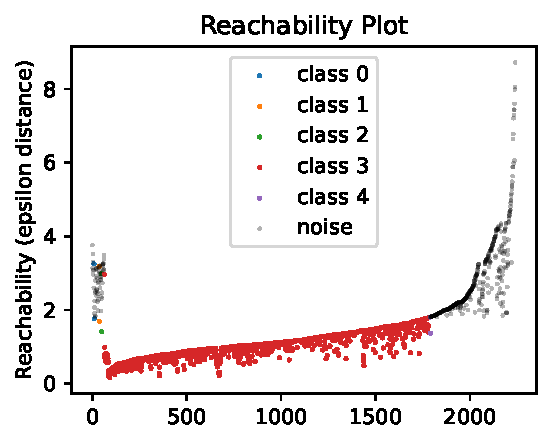
\includegraphics[width=6.5cm]{images/OPTICS/32x32/reachability_plot_32x32.pdf} }}%
    \qquad
    \subfloat[\centering The reachability plot of the documents preprocessed according to \autoref{pt:eigendocs} (i.e.\ \eigendocs{}).]{{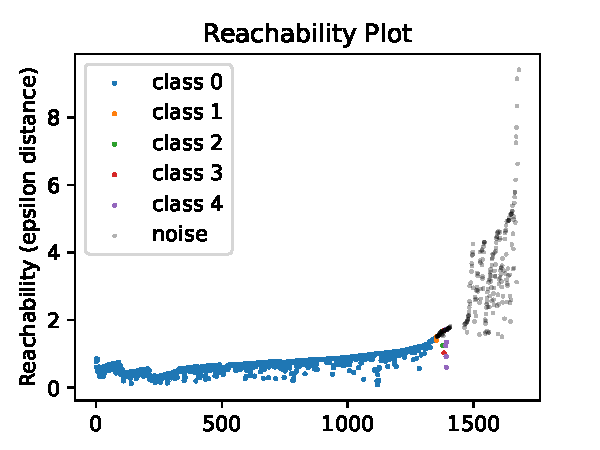
\includegraphics[width=7cm]{images/OPTICS/eigendocs/reachability_plot_eigendocs_13_dim.pdf} }}%
    \caption[Reachability distances]{The plot was created using the \acs*{optics} algorithm from the Python library scikit-learn.
    The underlying dataset consists of 2241 documents from the Bahamas leak.
    It shows the reachability distance of each document to its predecessor in the order list.}%
    \label{fig:reachability_plots}%
\end{figure}


% preprocessed images
\begin{figure}[!htp] % htp = hier (h), top (t), oder auf einer eigenen Seite (p).
    \centering
    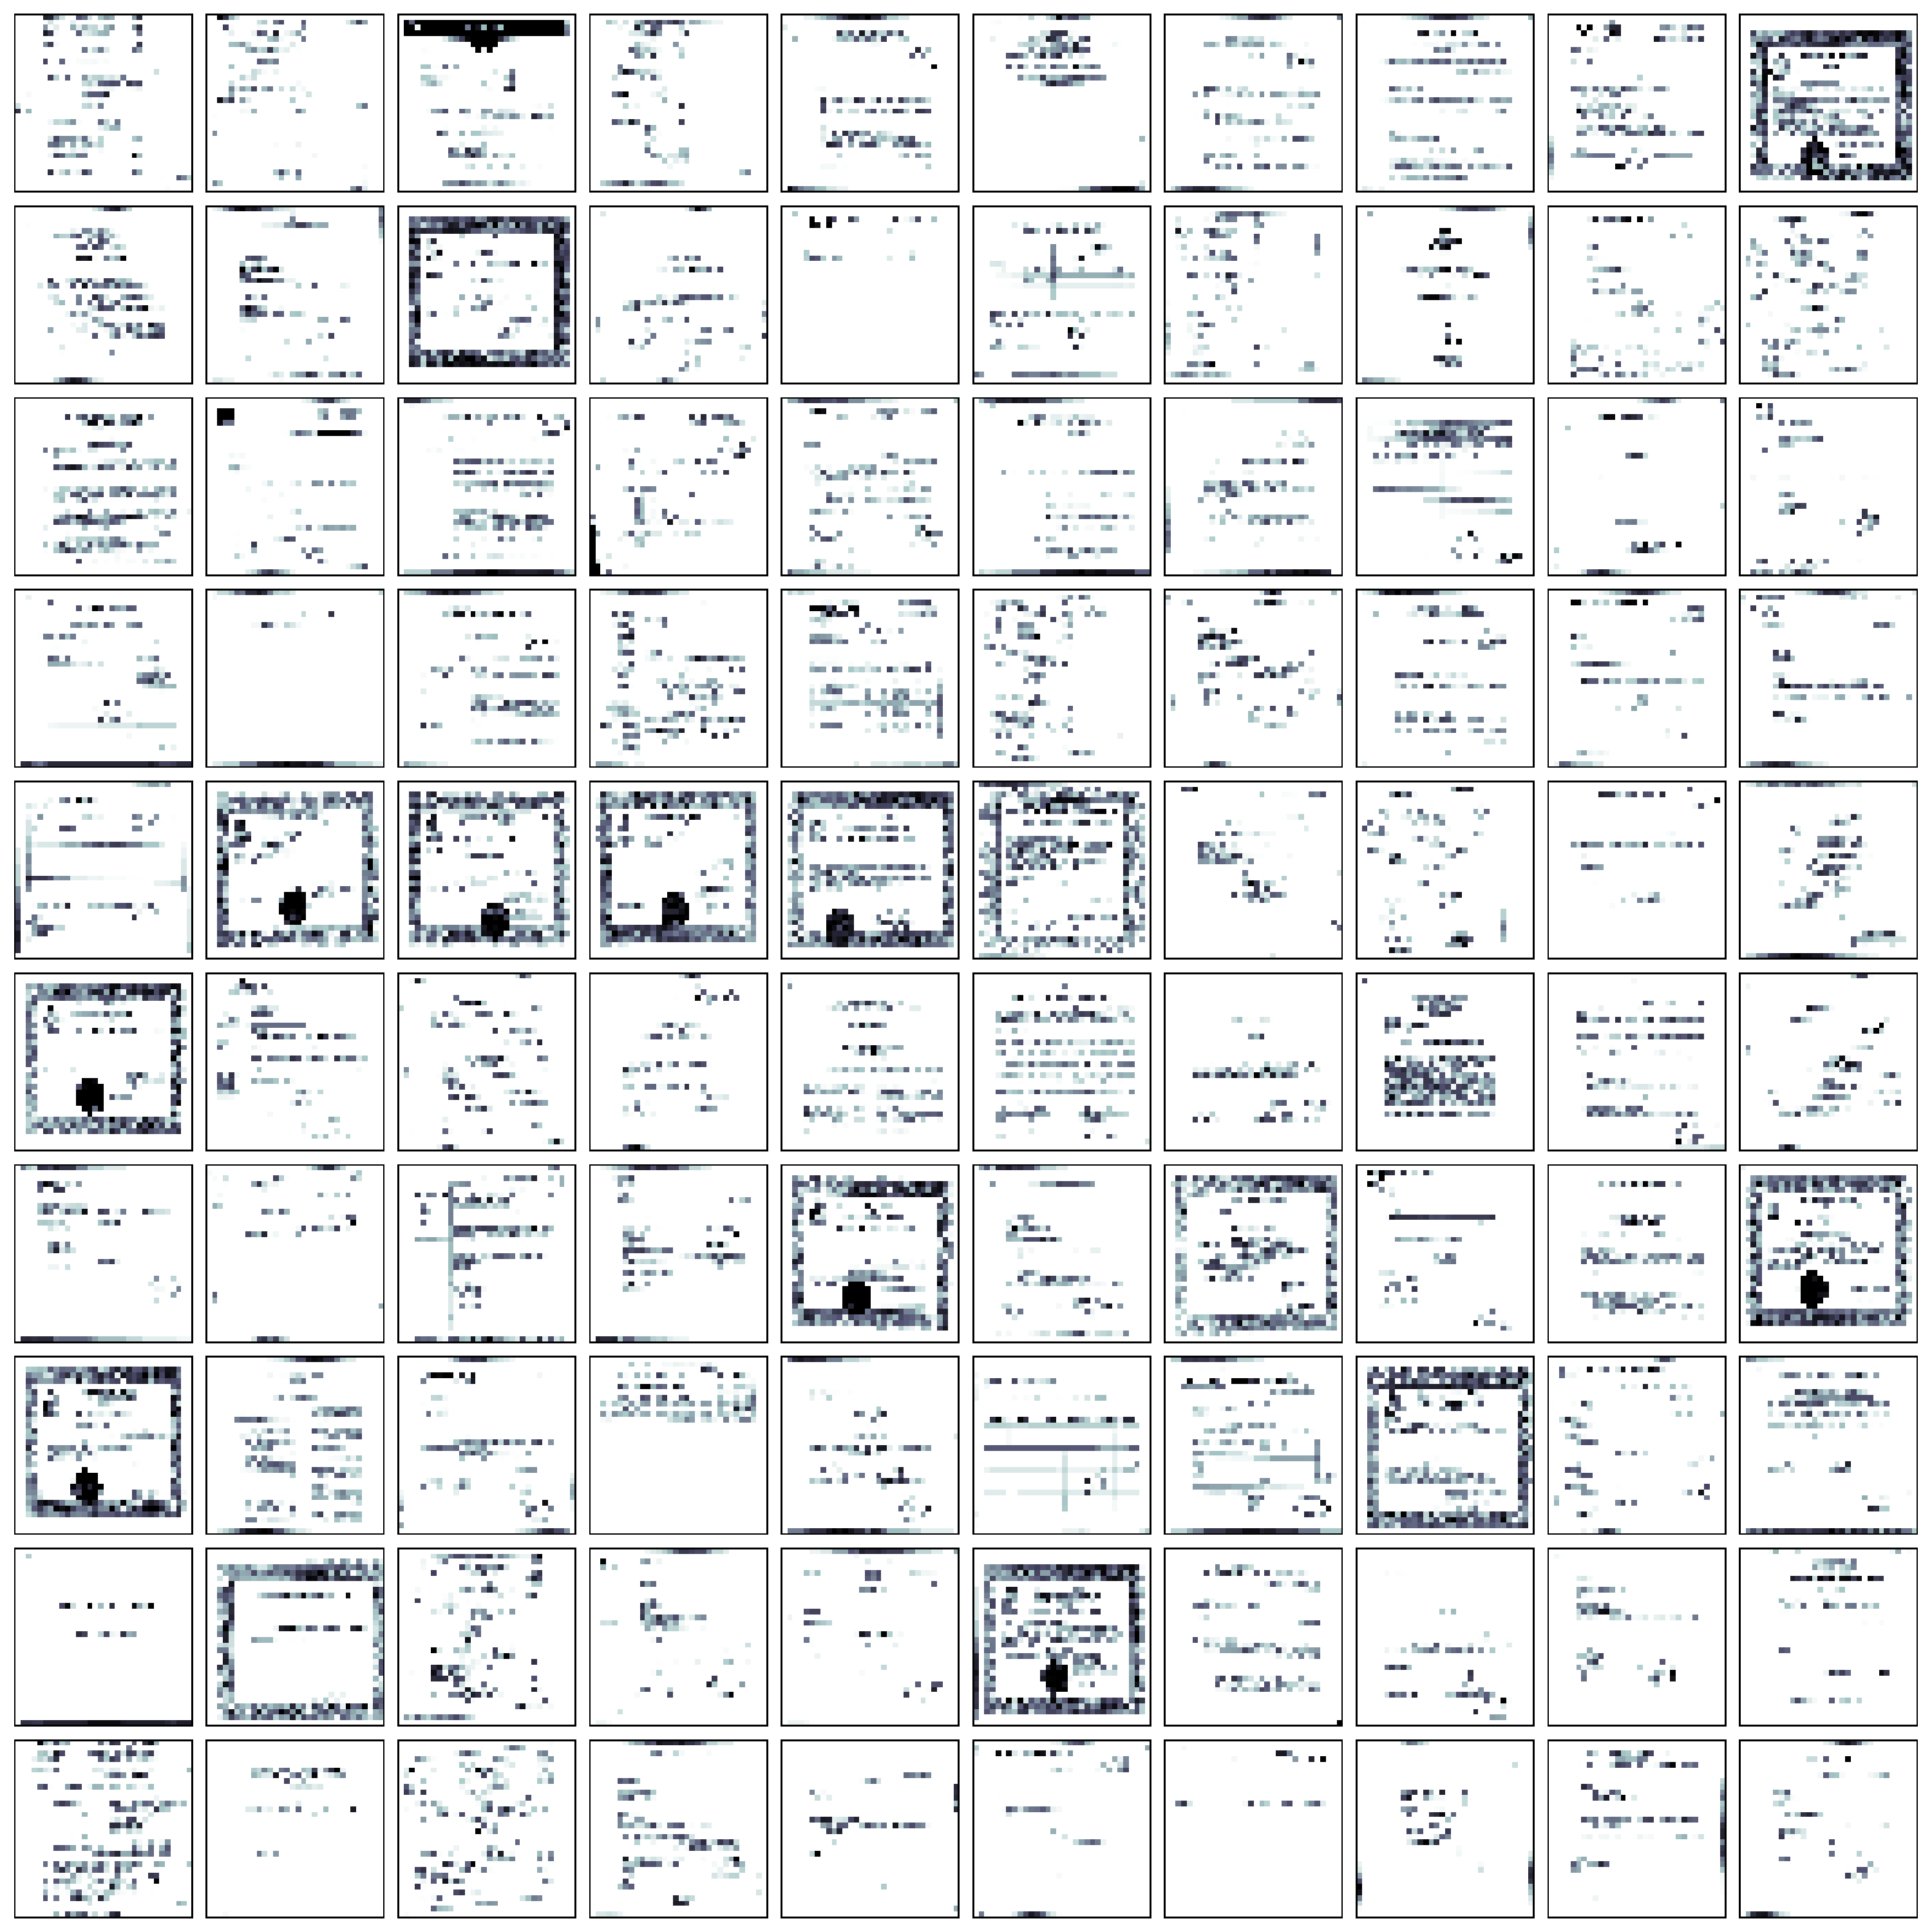
\includegraphics[width=1\textwidth]{images/OPTICS/32x32/preprocessed_docs.pdf}
    \caption[Preprocessing to 32x32 normalized greyscale pixels]{Preprocessing of 100 documents to 32x32 normalized greyscale pixels.
    }
    \label{fig:preprocessed_docs_32x32}
\end{figure}

%The resulting clusters are displayed in \autoref{fig:optics_cluster}.


\begin{listing}[!htp]
    \begin{minted}{python3}
        optics_model = OPTICS(cluster_method='dbscan', min_samples=2, max_eps=10, 
            eps=1.5)
    \end{minted}
    \caption[Initialization of the \ac{optics} model]{Initialization of the \ac{optics} model.
    The minimum number of samples \texttt{min\_samples} in a cluster corresponds to \textit{minPts}.
    }
    \label{lst:optics_model}
\end{listing}

% code
The configurations used when initializing an \ac{optics} model greatly influence the clusters returned.
The parameter \texttt{max\_eps} is infinity by default but can be specified by the user to reduce complexity and runtime.
According to literature, \texttt{max\_eps} should be big enough to include almost all points in a single cluster.
The way the reachability plot is used to extract clusters is dependent on the \texttt{cluster\_method}. 
One can choose either \texttt{dbscan} or \texttt{xi} as a clustering method.
The parameters \texttt{min\_samples} and \texttt{eps} influence the cluster sizes and number of clusters found for a given clustering approach.
The value of \texttt{eps} defines the distance between two points to still be considered neighbours 
and can be chosen by consulting the reachability plot which is displayed in \autoref{fig:reachability_plots}.
The code to initialize an exemplary \ac{optics} model is displayed in \lst{lst:optics_model}.
